\section{Computational evidence and reproducibility}
\label{sec:computation}

The calculations serve three distinct purposes: exact finite
certification, independent numerical diagnostics, and exploratory
identity discovery. All proof-relevant interval decisions use integers
and rational endpoints. The moment diagnostics and Mellin audit use
arbitrary-precision floating-point arithmetic and are labeled accordingly.
The article's symbolic proofs establish the all-parameter statements.

\subsection{What was verified}

\begin{longtable}{@{}P{0.23\textwidth}P{0.47\textwidth}P{0.24\textwidth}@{}}
\toprule
Computation & Coverage and outcome & Logical role\\
\midrule
\endhead
Euler kernel checks & 2601 rational scalar cases, 2025 strict interior
cases, and 560 exact kernel/tail identities pass. & Implementation
audit of an analytic theorem.\\
Universal constant & Eleven rational-order grid enclosures imply
$C_*<57/50$; a separate 384-bit outward interval calculation certifies
the narrow $b_*$ and $C_*$ brackets. & Exact finite certificates, using
the inherited unique-maximum theorem.\\
Global gamma slope & All 256 dyadic subintervals replay successfully;
the smallest lower bound exceeds $7/4$. & Reproduction of the inherited
compact part of the slope proof.\\
Moment expansion & 24 cases at 60 working decimal digits cover balanced,
fixed-ratio, square-root, fixed, fractional, axis, and transition families.
& Independent quadrature diagnostics.\\
Lerch mesh & Exact Sturm isolation for $2\le n\le12$; six gamma-moment
positive controls and one rejected negative control. & Finite improved
thresholds and implementation audit.\\
Shuffle matrices & Exact factorizations, unimodularity, determinants,
Smith factors and denominator checks for $1\le m\le20$; the short
weight-eleven row identity also passes. & Finite audit of the all-$m$
integer proof.\\
Gaussian candidates & Both retained normalized residuals lie strictly
inside $(-10^{-650},10^{-650})$; the rejected $S_{12}$ vector is separated
from zero. & Exact proximity and exact rejection, respectively.\\
Independent $S_{10}$ audit & 120-digit Mellin quadrature gives a normalized
residual about $3.49\times10^{-121}$. & Independent normalization check;
no rigorous quadrature error asserted.\\
\bottomrule
\end{longtable}

\subsection{Interpreting the diagnostic figures}

\begin{figure}[htbp]
\centering
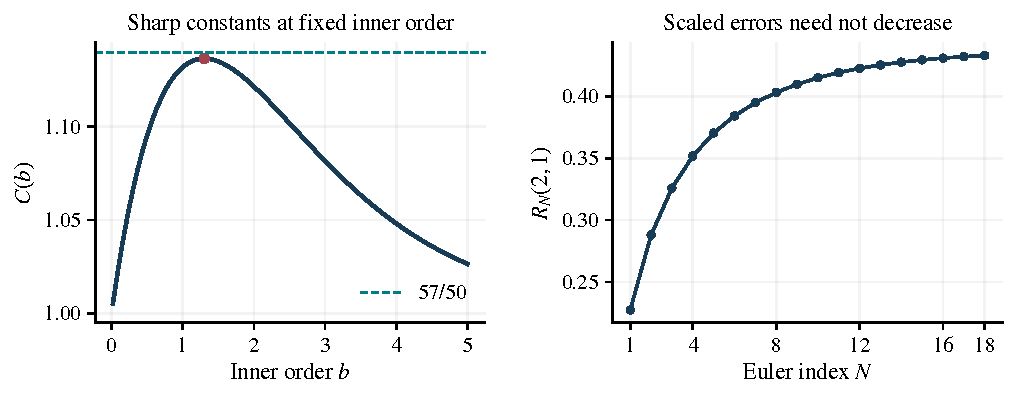
\includegraphics[width=\textwidth]{figures/euler_constants.pdf}
\caption{Left: the inner-order constant $C(b)$ and its unique maximum,
with the convenient rational budget $57/50$. Right: a finite diagnostic
plot of the scaled errors $R_N(2,1)$. Its initial increase is certified
symbolically by Proposition~\ref{prop:scaled-error-counterexample}; the
plot is not used to prove a global shape or to identify its eventual
maximum. The curves are numerical illustrations of proved bounds.}
\label{fig:euler}
\end{figure}

\begin{figure}[htbp]
\centering
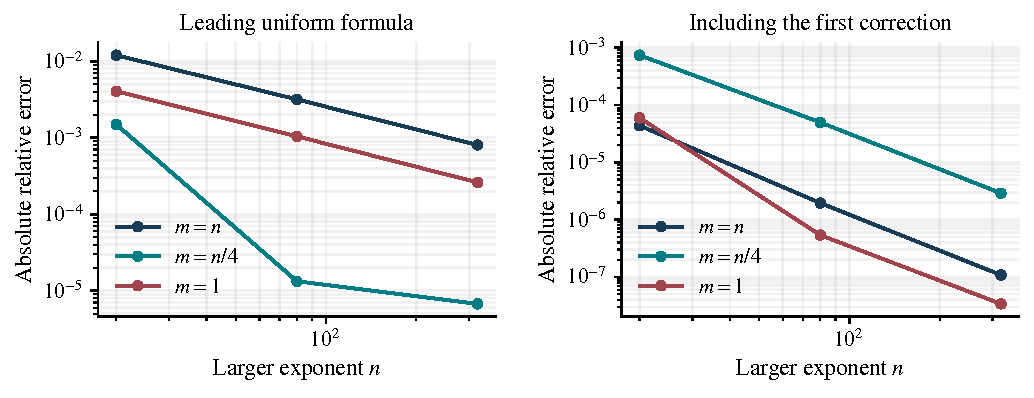
\includegraphics[width=\textwidth]{figures/uniform_moment_errors.pdf}
\caption{Absolute relative errors in the all-ratio moment approximation,
before and after the first correction, for three of the seven tested
parameter families. The reference values are computed by quadrature in
$t=-\log x$, independent of the inverse-coordinate saddle construction.
The first correction generally improves accuracy at sufficiently large
exponents; cancellation can make an uncorrected finite case unusually
accurate, so pointwise improvement at every input is not a theorem.}
\label{fig:moments}
\end{figure}

For example, for $m=n=20,80,320$, the corrected relative errors have
absolute values approximately
$4.39\times10^{-5}$, $1.95\times10^{-6}$, and $1.08\times10^{-7}$.
For $m=n/4$ the corresponding values are approximately
$7.41\times10^{-4}$, $4.98\times10^{-5}$, and $2.89\times10^{-6}$.
These finite values illustrate the theorem but cannot determine the
uniform error constant. The axis diagnostic also checks against the
source's strict factorial comparison; it does not incorrectly substitute
$M_{n,0}=\Gamma(n+1)$ as an exact identity.

\begin{figure}[htbp]
\centering
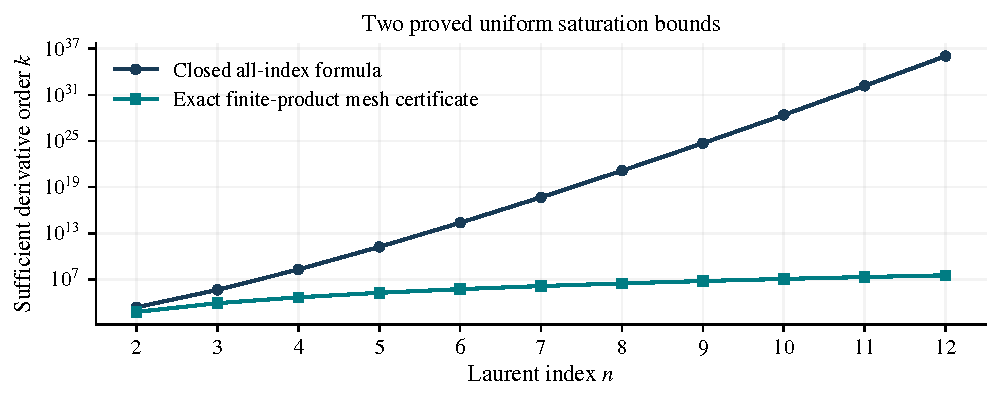
\includegraphics[width=0.86\textwidth]{figures/lerch_thresholds.pdf}
\caption{Two sufficient Lerch saturation thresholds: the explicit
all-index formula and the improved bounds obtained from exact finite
Sturm isolation of $B_n$. The vertical axis is logarithmic. The displayed
integers are consequences of the same proved sign-transfer criterion;
they are not estimates of the sharp transition. In particular the known
index-two threshold is $1$, below both curves.}
\label{fig:lerch}
\end{figure}

\subsection{A portable replay protocol}

The archive provides \code{code/verify_all.py}. The default command
runs the exact certificates and finite matrix audit. It records commands,
exit status, elapsed time, and output hashes in a replay manifest. A
\code{--numerical} option additionally recomputes the 24 moment diagnostics;
the independent 120-digit Mellin audit has its own optional command.
No verification command requires network access or a checkout of the
source repository. The inherited gamma-slope program is copied unchanged
and explicitly attributed.

The Gaussian input is \code{code/gaussian/gaussian_candidates.json}.
The historical discovery files retain both the unsuccessful first
weight-thirteen search and the successful higher-precision search.
Their role is audit history; the verifier reads only the canonical
retained/rejected records. This avoids inadvertently promoting an obsolete
integer vector when integrating the work.

LaTeX compilation uses \code{code/build_article.py} to concatenate the
preamble, ordered section fragments and bibliography into a complete
\code{article.tex}, then \code{latexmk -pdf article.tex}. The final
article source can be compiled without Python when the bundled figure
PDFs are present. Figure regeneration is optional and uses the saved
diagnostic data. The archive includes a file-hash manifest and the exact
source revision for every inherited dependency.

\FloatBarrier
